\begin{problem}
Write
\end{problem}

\begin{solution}
The operator is not linear. Let $f(x) = \sin (x), g(x) = \cos (x)$ and consider the space $\mathcal{P}_0 \subset \mathcal{C}[0, \pi/2]$. It is easy to see that the best minimax approximation to both of these functions is $p(x) = 1/2$ as it satisfies the characterization theorem. However if we take $f(x)+g(x)$ we get that the best minimax approximation is $p(x) = \sin(\pi/4)+\cos(\pi/4)>1$. thus the property:
\begin{equation*}
X(f+g) = X(f) + X(g)
\end{equation*}
is not fulfilled.
\begin{figure}[h]
\centering 
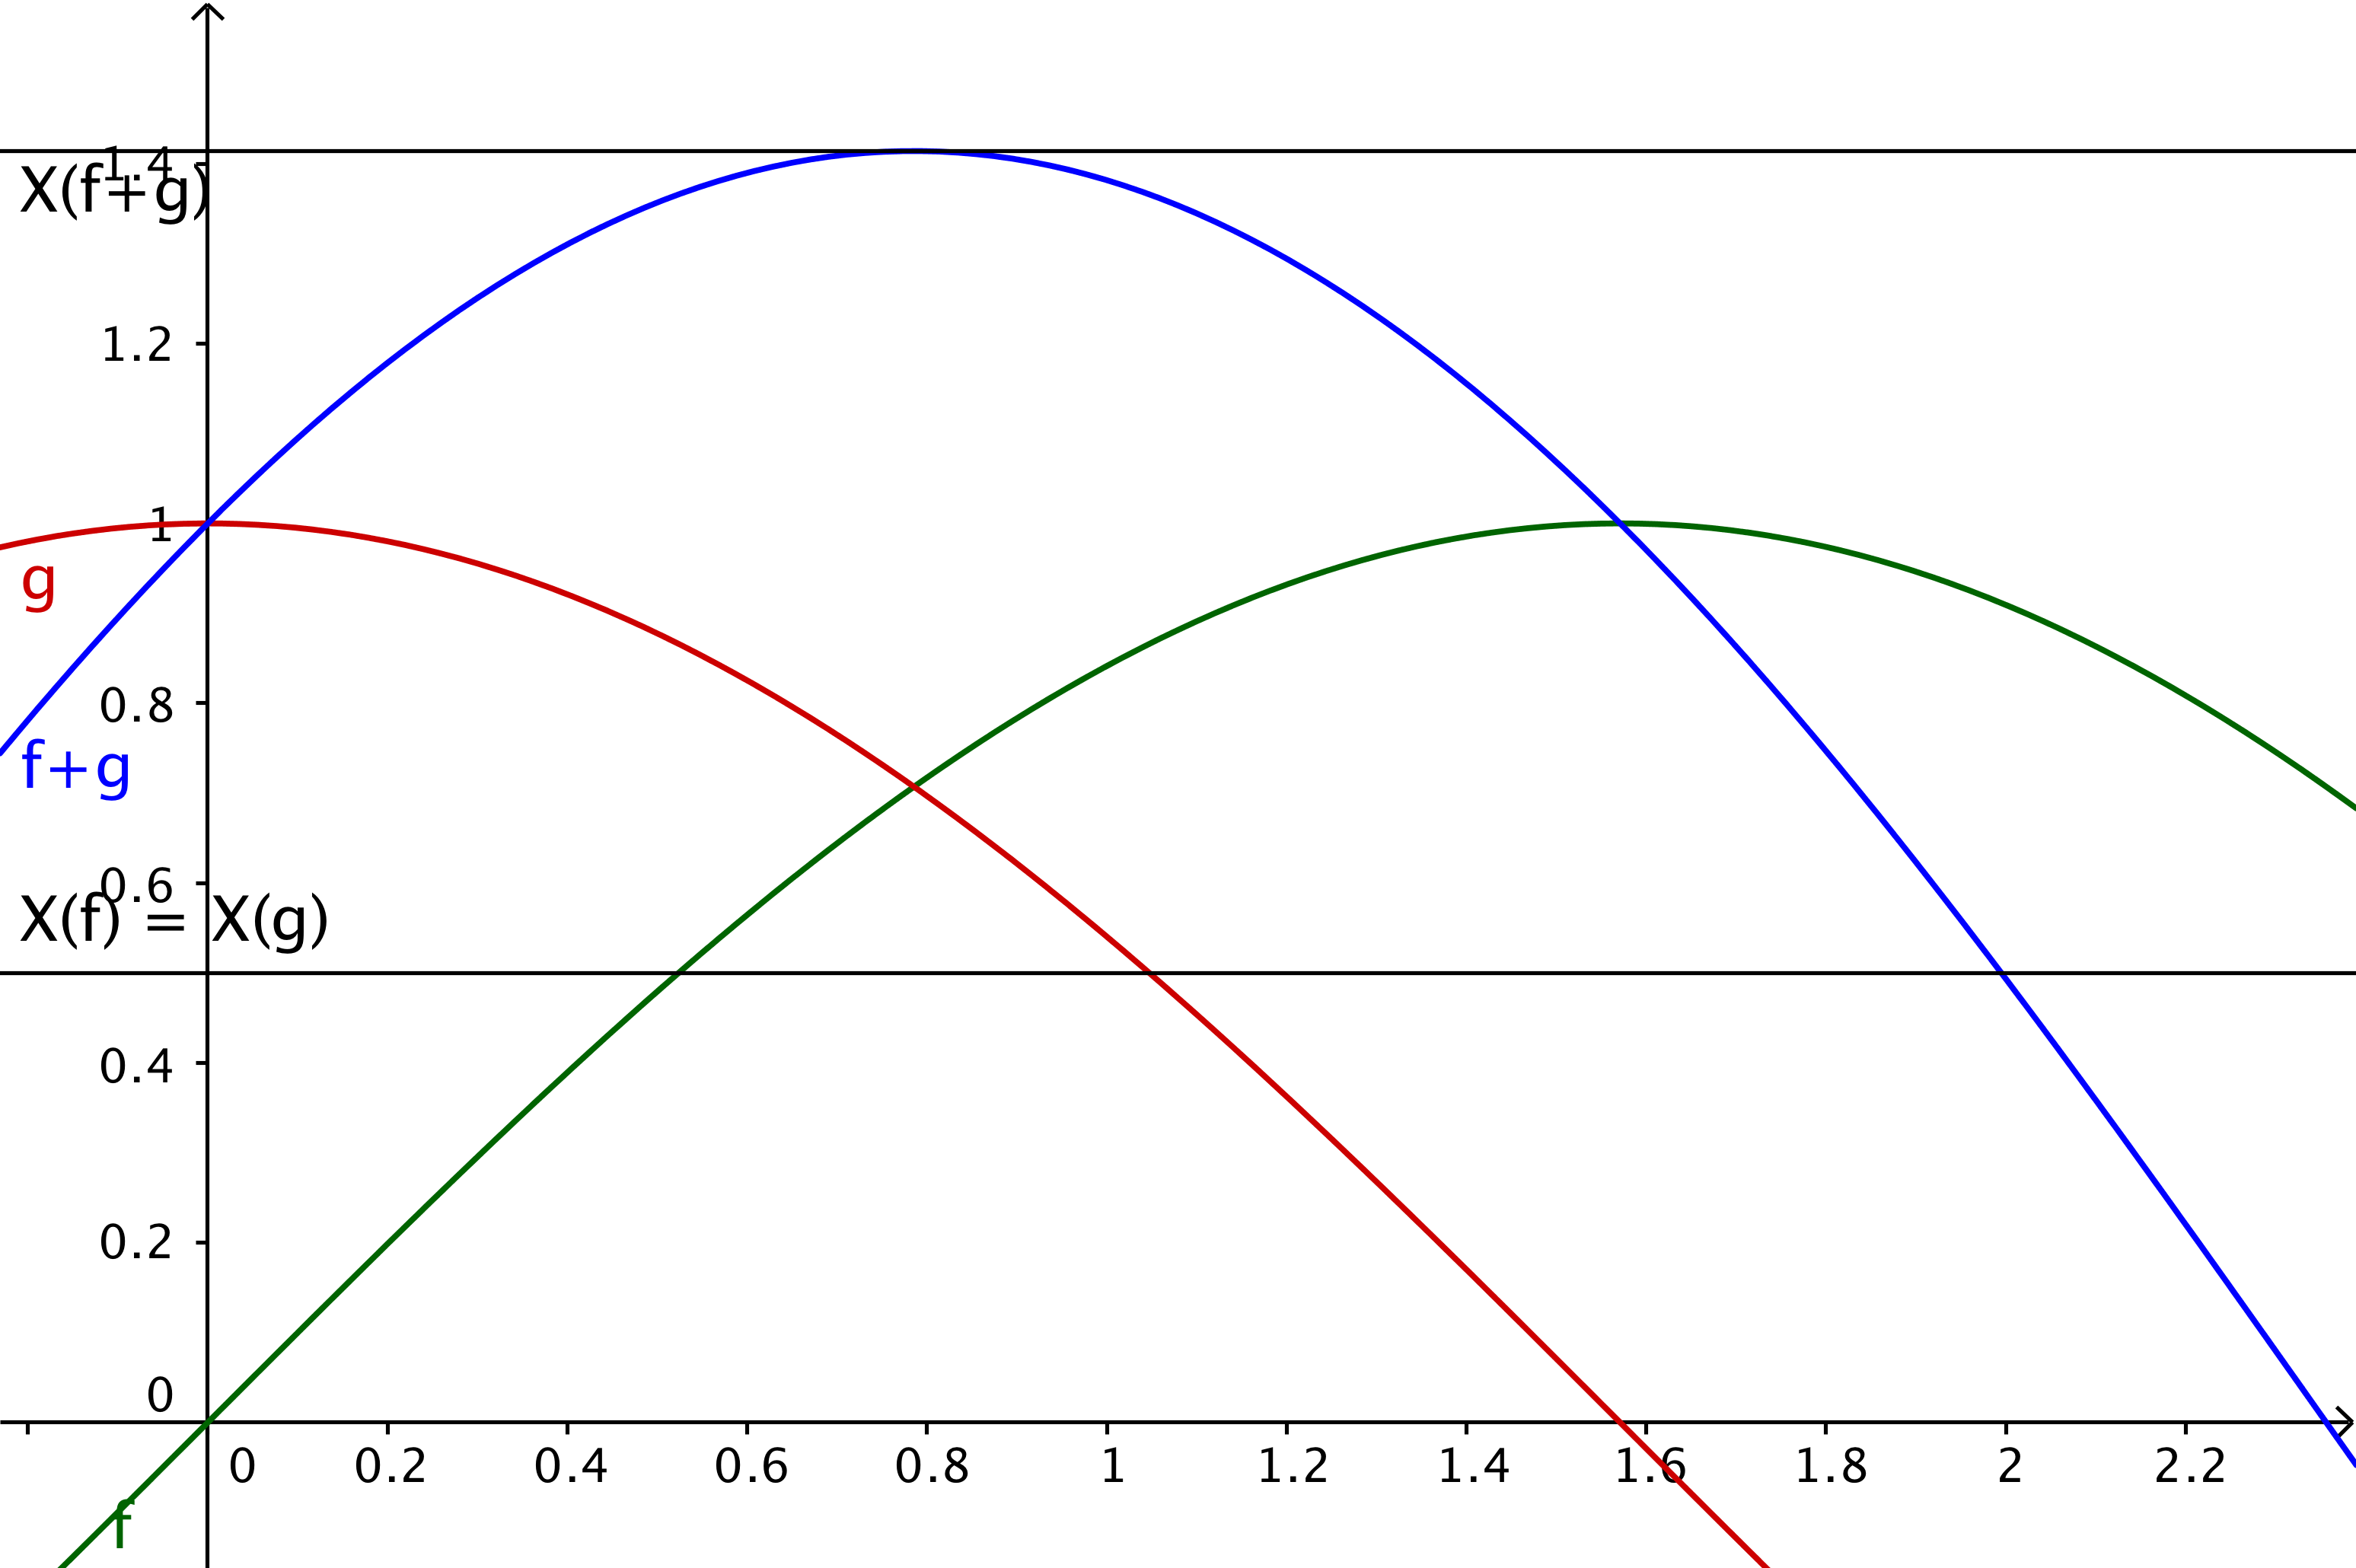
\includegraphics[scale = 0.5]{figtask6.png}
\caption{Plot of the functions and their best minimax approximations}
\label{figtask6}
\end{figure}

\end{solution}